\chapter{Simulation Design}
The simulation is a very important part of the project. It is required to provide the basic functionality of a LTE network. For simplicity the simulation was broken down into two main components; the mobile (UE) and the base station (eNodeB). Due to the project revolving around the handover process in LTE, it made sense for the two main components of the simulation to be the mobile and the base station; it is the mobile that triggers the measurement report and the base station that makes the decision on whether a handover should take place or not. Since the A3 event trigger (Table~\ref{tab:trigger}) is the most common it was decided that it would be the only trigger implemented in the simulation to reduce the complexity within the simulation.

It was required for the mobile to be able to move freely around a group of base stations. It was decided that this movement should be random because if any machine learning algorithm can handle random movement then it should also be able to handle regimented movement. The movement that the mobile follows is defined by a Mobility Model and the choice of mobility model is explained in Section~\ref{mobility}. It was decided that when a UE would get to the point where its next step would move it beyond the bounds of the simulation area that it would just move in the reflected direction away from the wall.

In wireless communications the received signal strength from a transmitter degrades the further away from the transmitter the receiver is. A propagation model can be used to define the way in which the signal strength degrades. The propagation model is very important to the simulation as it will define how far away from a base station the mobile can be without dropping the call. A comparison and explanation of the choice of propagation model can be seen in Section~\ref{propagation}.
\section{Simulation Parameters}
Within the simulation there are many variable parameters that need to be assigned values. Such parameters are: the height of the base stations, the height of the UEs, the dimensions of the simulation area and the positioning of the base stations. Other parameters that also needed to be considered are the number of base stations and the number of UEs. The type of environment also had to be chosen; whether the simulation would be within a rural, urban, small city, medium city or large city environment.

The type of environment was decided to be a medium sized city. It was decided that the height of any UE would be $1 m$ as it would normally be in the possession of a human being. The height of any base station would be $60 m$ because base stations are either placed upon tall buildings or structures so that they produce better coverage. Since it was decided that the environment would be a medium sized city, this height made sense since there would be some large multi-storey building. The simulation area and positioning of the base stations both depended on the propagation model used and the area of coverage that could be expected from it. The decision of the propagation model used can be found in Section~\ref{propagation}. From Figure~\ref{fig:prop} it was found that for the chosen propagation model the Path Loss would reach the LTE noise floor of $-97.5 dB$ at around $2 km$. Therefore, from this it was decided that the area for the simulation would be $6 km$ by $6 km$. It was then decided that 9 base stations would provide good coverage in this area. Each of these base stations will also have there own Q-Learning agent since each base station has there own unique TTT and hys values. The base stations were placed in the following locations and the coverage can be seen in Figure~\ref{fig:cov}.
\begin{enumerate}
\item X Co-Ordinate: 500.0, Y Co-Ordinate: 500.0
\item X Co-Ordinate: 3000.0, Y Co-Ordinate: 0.0
\item X Co-Ordinate: 5500.0, Y Co-Ordinate: 500.0
\item X Co-Ordinate: 0.0, Y Co-Ordinate: 3000.0
\item X Co-Ordinate: 3000.0, Y Co-Ordinate: 3000.0
\item X Co-Ordinate: 6000.0, Y Co-Ordinate: 3000.0
\item X Co-Ordinate: 500.0, Y Co-Ordinate: 5500.0
\item X Co-Ordinate: 3000.0, Y Co-Ordinate: 6000.0
\item X Co-Ordinate: 5500.0, Y Co-Ordinate: 5500.0
\end{enumerate}
\begin{figure}[H]
  \begin{center}
    	  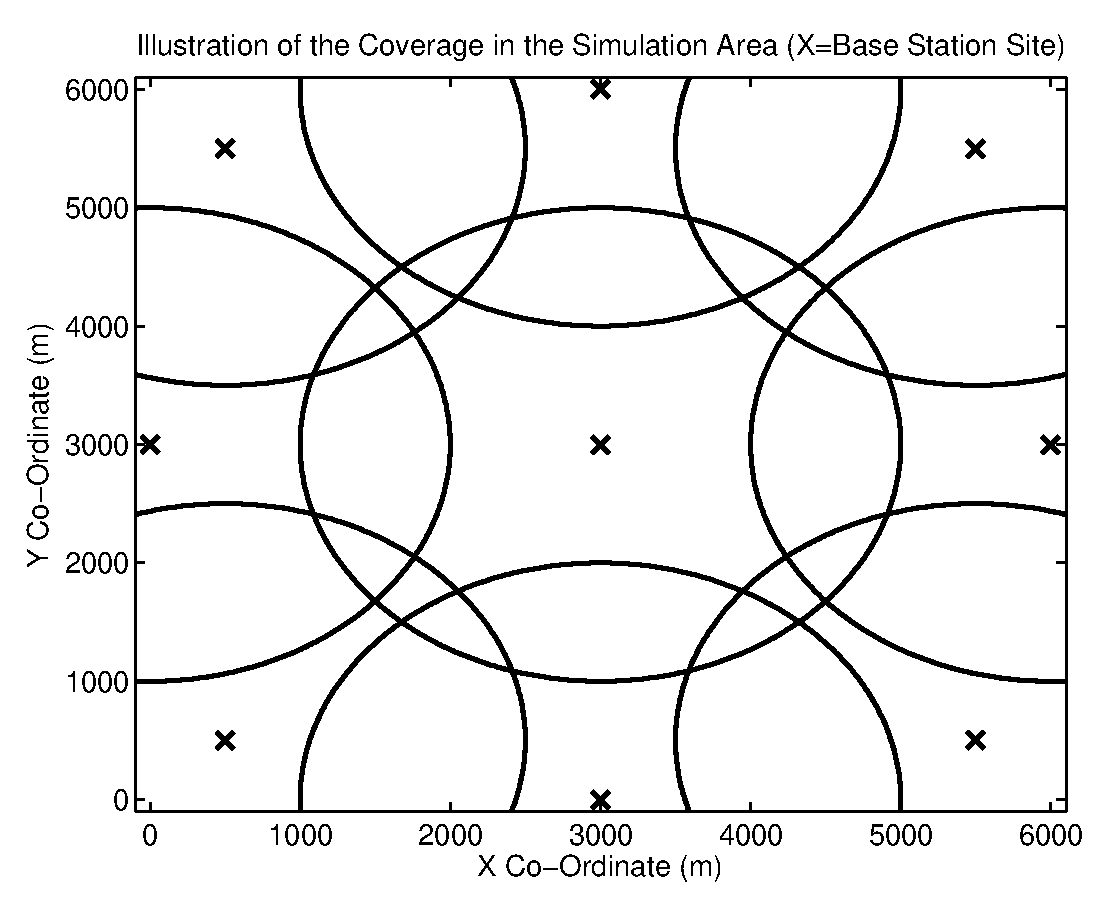
\includegraphics[width=0.75\textwidth]{figures/simulation/coverage.eps}
    \end{center}
    \caption{Illustration of Coverage within the Simulation Area.}
    \label{fig:cov}
\end{figure}

Finally, it was decided that 10 UEs would be used in the simulation because this would allow for the learning done by the Q-Learning agents to happen faster than if there were just 1 UE. The UEs would also start on top of different base stations so that they will start in different places allowing for the Q-Learning agent for each base station to start learning straight away without having to wait for a UE to move into range, as at least 1 UE will start on top of it.
\section{Discrete Event Simulation}
The concept of time is very important in real world simulations. A popular method for creating this concept of time is \ac{DES}. It works on the basis of a scheduler where events, to be processed at a certain time, are passed to the scheduler and the scheduler then passes the event on to be processed. The way that \ac{DES} creates the concept of time is by allowing events passed in the scheduler to have a time that it should be processed at, the scheduler will keep all the events that are currently still to be processed in an ordered list, the scheduler will then `jump' to the time the first event in the list is to be processed at and passes the event on to be processed. The process of `jumping' to the next time that the first event in the list is to be processed at is what gives \ac{DES} the concept of time.

Another advantage of \ac{DES} is that the passing of events from the scheduler not only gives a concept of time but it also allows for a message to be sent with the event to tell a different part of the simulation what to do at a given time. This message can also pass parameters for the other part of the simulation to use.

\section{Mobility Model}\label{mobility}
A mobility model defines the way in which an entity will move. For the purposes of the simulation the mobility model used needed to be random in nature. After some research it was decided that the mobility model to be used in the simulation would either be the Random Direction or Random Waypoint model because they are two of the most popular random mobility models.~\cite{roy2010handbook}
\subsection{Random Direction Model}
The Random Direction Model is defined as follows:
\begin{enumerate}
\item Select a direction randomly between 0 and 359 degrees.
\item Select a random speed to move at.
\item Select a random duration to move for.
\item Move in the selected direction at the selected speed for the selected duration.
\item Repeat until termination.
\end{enumerate}
\subsection{Random Waypoint Model}
The Random Waypoint Model is defined as follows:
\begin{enumerate}
\item Randomly select the co-ordinates for a point within the environment.
\item Select a random speed to move at.
\item Select a random length of time to pause for when the destination is reached.
\item Move towards the selected co-ordinates at the selected speed
\item Pause for the randomly selected length of time.
\item Repeat until termination.
\end{enumerate}

It was decided that the Random Direction Model would be used in the simulation because the Random Waypoint Model has the problem that it is possible to select the co-ordinates of a point very close to where you begin and then pause for a long period time. The possibility of that happening is undesirable within the simulation. Random Direction does not have this problem and it is also possible to set boundaries on the parameters to make sure that a minimum distance is travelled.~\cite{roy2010handbook}

\section{Propagation Model}\label{propagation}
A propagation model defines how the received signal from a transmitter decays the further from the transmitter you are. There are many different models available, all with different functions and purposes. After some research three models were considered; the Okumura-Hata Model, the Egli Model and the Cost231-Hata Model.
\subsection{Okumura-Hata Model}
The Okumura-Hata model is very popular for simulating transmissions in built up areas. Equations~\ref{eq:okumura},~\ref{eq:oksmall} and~\ref{eq:oklarge} show the formulas for the model.
\begin{equation}\label{eq:okumura}
L_{u}=69.55+26.16log_{10}f-13.82log_{10}h_{B}-C_{h}+[44.9-6.55log_{10}h_{B}]log_{10}d 
\end{equation}
For small or medium sized cities:
\begin{equation}\label{eq:oksmall}
C_{H}=0.8+(1.1log_{10}f-0.7)h_{m}-1.56log_{10}f
\end{equation}
For large cities.
\begin{equation}\label{eq:oklarge}
C_{H}=
	\begin{cases}
	8.29(log_{10}(1.54h_{M}))^{2}-1.1 & \mbox{if } 150 \leq f \leq 200 \\
	3.2(log_{10}(11.75h_{M}))^{2}-4.97 & \mbox{if } 200 < f \leq 1500
	\end{cases}
\end{equation}
Where:
\begin{itemize}
\item $Lu$ is the path loss ($dB$).
\item $H_{B}$ is the height of the base station antenna $30$ to $200 m$.
\item $H_{R}$ is the height of the mobile antenna $1$ to $10 m$.
\item $f$ is the frequency of the transmission $150$ to $1500 MHz$.
\item $C_{H}$ is the antenna correction factor.
\item $d$ is the distance between the base station and the mobile $1$ to $20 km$.
\end{itemize}
\subsection{Egli Model}
The Egli Model was another model that was considered for the simulation. Equations~\ref{eq:eglis} and~\ref{eq:eglil} shows the formulas for the model.

If $h_{m}$ is less than or equal to $10 m$ height:
\begin{equation}\label{eq:eglis}
P_{L}(dB) = 20log_{10}f_{c}+40log_{10}d-20log_{10}h_{b}+76.3-10log_{10}h_{m}
\end{equation}
If $h_{m}$ is greater than or equal to $10 m$ height:
\begin{equation}\label{eq:eglil}
P_{L}(dB) = 20log_{10}f_{c}+40log_{10}d-20log_{10}h_{b}+83.9-10log_{10}h_{m}
\end{equation}
Where:
\begin{itemize}
\item $P_{L}(dB)$ is the path loss ($dB$).
\item $h_{B}$ is the height of the base station antenna ($m$).
\item $h_{M}$ is the height of the mobile antenna ($m$).
\item $d$ is the distance between the base station and the mobile ($m$).
\item $f$ is the frequency of the transmission $3 MHz$ to $3000 MHz$.
\end{itemize}
\subsection{Cost231-Hata Model}
The Cost231-Hata model is an extension of the Okumura-Hata to work for frequencies between 1.5 GHz and 2 GHz. The formulas for this model can be seen in Equations~\ref{eq:cost},~\ref{eq:costahr} and~\ref{eq:metro}.
\begin{equation}\label{eq:cost}
L=46.3+33.9logf-13.82log{h_{B}}-a(h_{R})+[44.9-6.55log{h_{B}}]log{d}+C
\end{equation}
\begin{equation}\label{eq:costahr}
a(h_{R})=(1.1log{f}-0.7)h_{M}-(1.58log{f}-0.8)
\end{equation}
\begin{equation}\label{eq:metro}
C=
	\begin{cases}
	0 dB & \mbox{for medium cities and suburban areas} \\
	3 dB & \mbox{for metropolitan areas}
	\end{cases}
\end{equation}
Where:
\begin{itemize}
\item $L$ is the path loss ($dB$).
\item $f$ is the frequency of the transmission $1500$ to $2000 MHz$.
\item $h_{B}$ is the height of the base station antenna $30$ to $200 m$.
\item $h_{M}$ is the height of the mobile antenna $1$ to $10 m$.
\item $d$ is the distance between the base station and the mobile $1$ to $20 km$.
\item $a(h_{R})$ is the antenna correction factor.
\end{itemize}
A comparison of the three propagation models can be seen in Figure~\ref{fig:prop}. For the graphs the height of the mobile was said to be $1 m$, while the height of the base station was said to be $60 m$. The frequencies used in the models were $2000 MHz$ for the Egli and Cost231-Hata models and $1500 MHz$ for the Okumura-Hata model. These values for the propagation models are then taken away from a base station transmit power of $48 dB$ so that the graphs are an estimate of the signal strength that would be received by a mobile at any distance up to $20 km$.
\begin{figure}[H]
  \begin{center}
    	  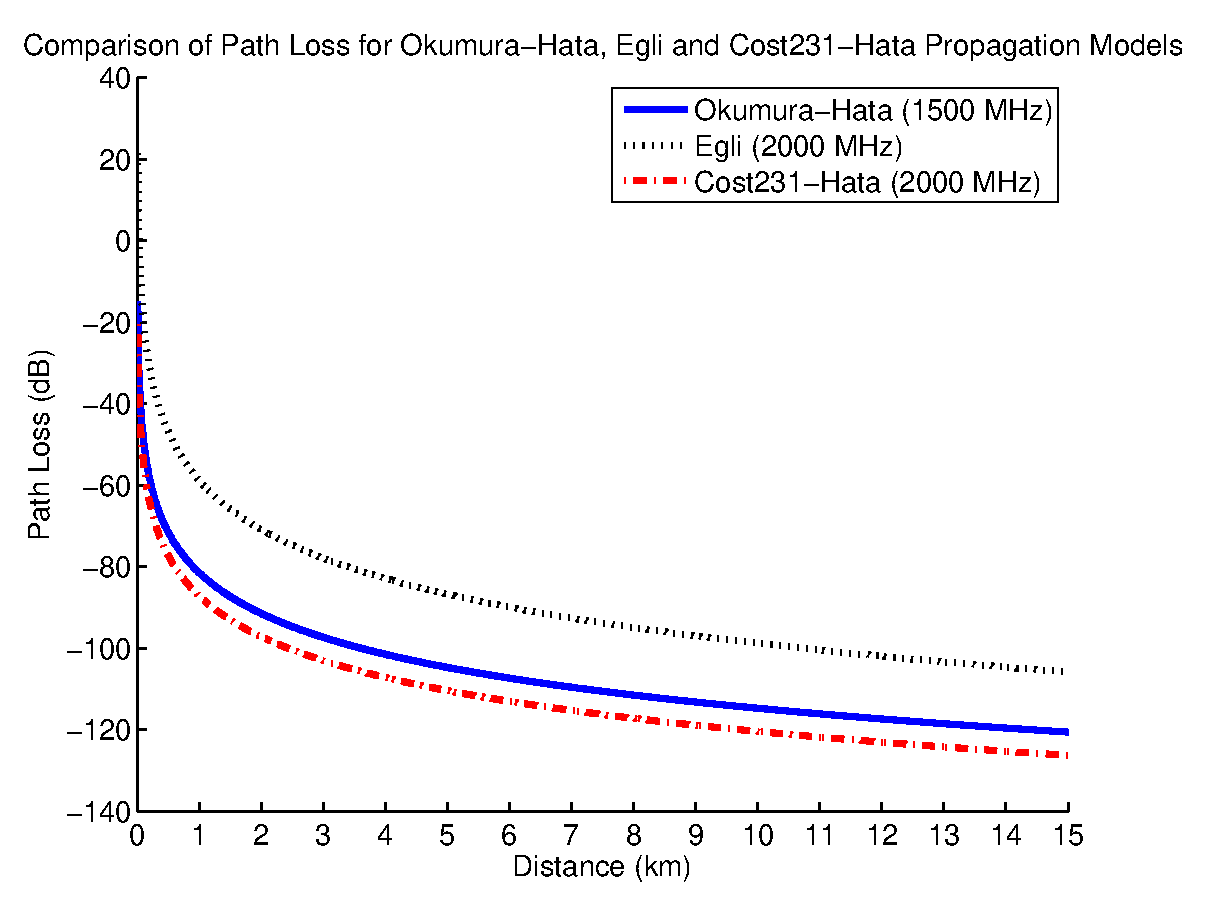
\includegraphics[width=0.75\textwidth]{figures/simulation/prop.eps}
    \end{center}
    \caption{Graph of different Propagation Models.}
    \label{fig:prop}
\end{figure}
After comparing the three models above it was decided that the Cost231-Hata Model would be the one used in the simulation due to it working with frequencies up to $2000 MHz$ (which is the minimum operating frequency of LTE) unlike the Okumura-Hata model which only works up to $1500 MHz$. The Cost231-Hata Model was also picked over the Egli Model because the Egli Model used more parameters that would add more complexity to the simulation.~\cite{chebil2011comparison, shabbir2011comparison}

\section{Simulation Implementation}


\section{Simulation Testing}
It was very important for the simulation and Q-Learning algorithm to be tested so that there was confidence that they would produce the correct results when they were run. There are many different types of testing that can take place to ensure that a piece of software is working correctly. Testing methods that were used in this project include: Unit testing, Black Box testing and White/Clear Box testing.

Unit testing involves testing individual parts or processes of a program so that the stakeholders can be confident in them to be fit for use. The different parts of the simulation that were tested this way were the Mobility Model, handovers, drops, ping-pong's and the Q-learning algorithm changing the values of TTT and hys correctly.

Black Box testing involves making sure that a function works as required without any knowledge of the under laying code. This type of testing is performed by giving a function an input, and comparing the output from the function with a previously determined expected output.

White Box testing is used to make sure that the underlying code used in a function works as required. This type of testing is done by inserting print statements in the code to see how the respective variables are changing while the code is running. These are compared against previously determined expected values to confirm whether the function is working as intended.

The test cases used to test the simulation to make sure it was working correctly were: 
\subsection*{Movement:}
\begin{description}
\item[M001]	Positive X and Y movement.
\item[M002]	Positive X movement and Negative Y movement.
\item[M003]	Negative X movement and Positive Y Movement.
\item[M004]	Negative X and Y movement.
\item[M005]	Movement against left wall of simulation area.
\item[M006]	Movement against bottom wall of simulation area.
\item[M007]	Movement against right wall of simulation area.
\item[M008]	Movement against top wall of simulation area.
\end{description}
\subsection*{Path Loss:}
\begin{description}
\item[PL001]	Received Path Loss correct.
\end{description}
\subsection*{Network Functions:}
\begin{description}
\item[NF001]	Handovers working correctly.
\item[NF002]	Drops working correctly.
\item[NF003]	Ping-Pong's detected correctly.
\end{description}
\subsection*{Q-Learning:}
\begin{description}
\item[QL001]	Q-Values updated correctly.
\item[QL002]	Changing state correctly.
\item[QL003]	Changing TTT and hys values correctly.
\end{description}
After the simulation was tested using the test cases above it was decided that the simulation was functioning correctly and was fit for use. The results of all the test cases can be seen in Appendix~\ref{testing}.
